\section{步骤分析}
$\bullet$做音频信号时域图,由于蜂鸣干扰,时域图像如下:
\begin{figure}[H]
    \centering
    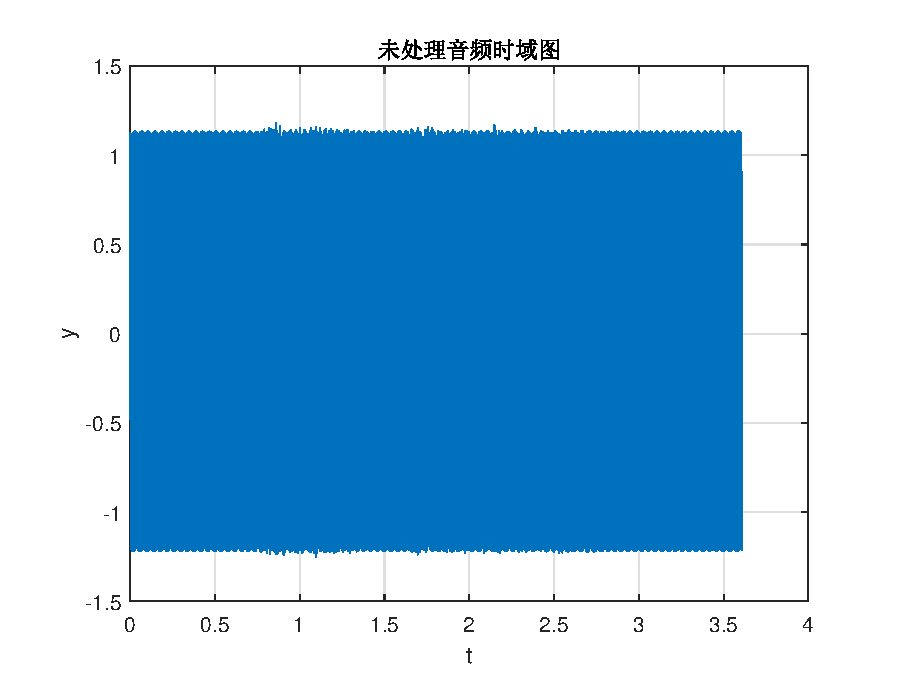
\includegraphics[width=8cm]{un-pict.eps}
    \caption{原音频信号时域图 }
\end{figure}
$\bullet$做音频信号频域图,并根据频域图像标记噪声频谱。\textit{此类噪声为单音噪声}\\\textit{单音噪声的消除首先考虑以某一幅度标准为限制,高于此幅度的进行滤除}
\begin{figure}[H]
    \centering
    \subcaptionbox{原音频信号频域图}{
        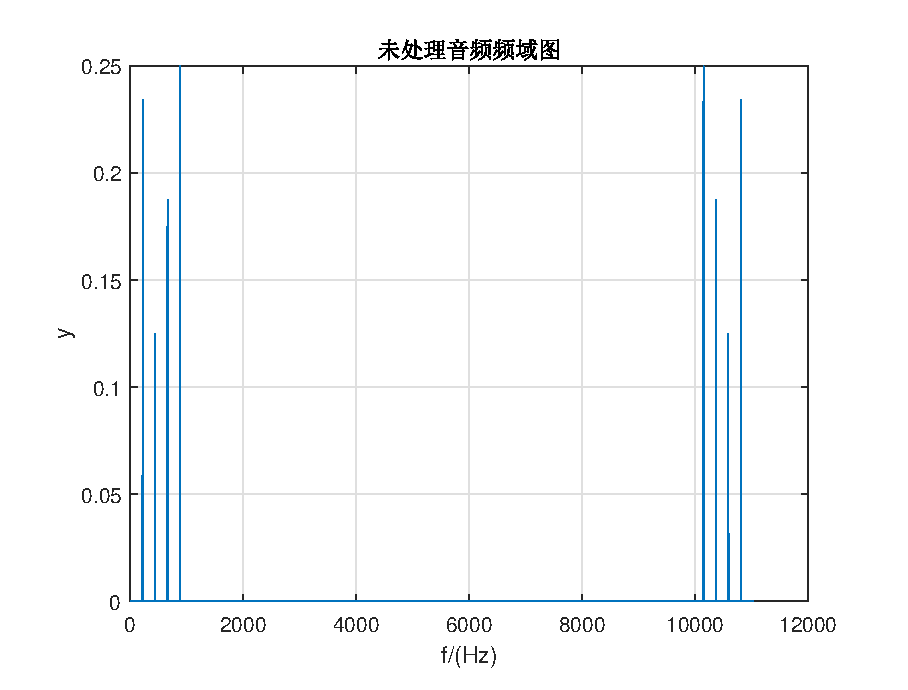
\includegraphics[width=11cm]{un-picf1.eps}	
    }
    \hfill 
    \subcaptionbox{原音频信号频域图-【标记噪声】}{
        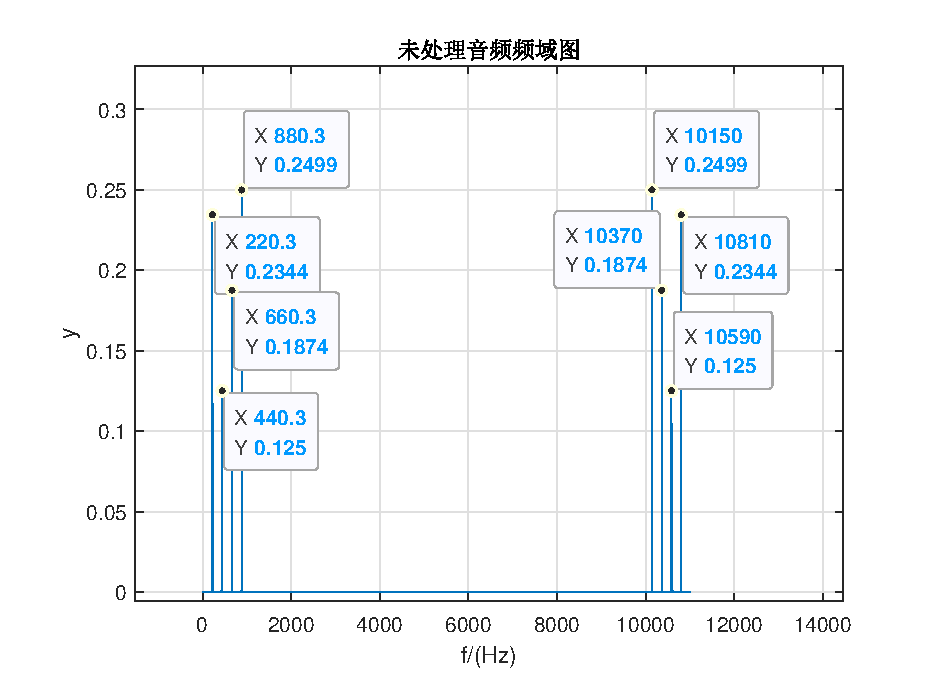
\includegraphics[width=11cm]{un-picf.eps}	
    }
    \caption{原音频信号频域图}
\end{figure}
\newpage
$\bullet$对音频信号进行初步处理。\textit{标记点y值:即为单音噪声滤除的幅度标准;标记点x值可判断出滤波器的上下限截止频率}\\
\indent 此时,已经可以消除绝大部分蜂鸣噪声,并辨析出该段音频在播放:\textit{‘这里是电子科技大学’}。

\begin{figure}[H]
    \centering
    \subcaptionbox{频域图}{
        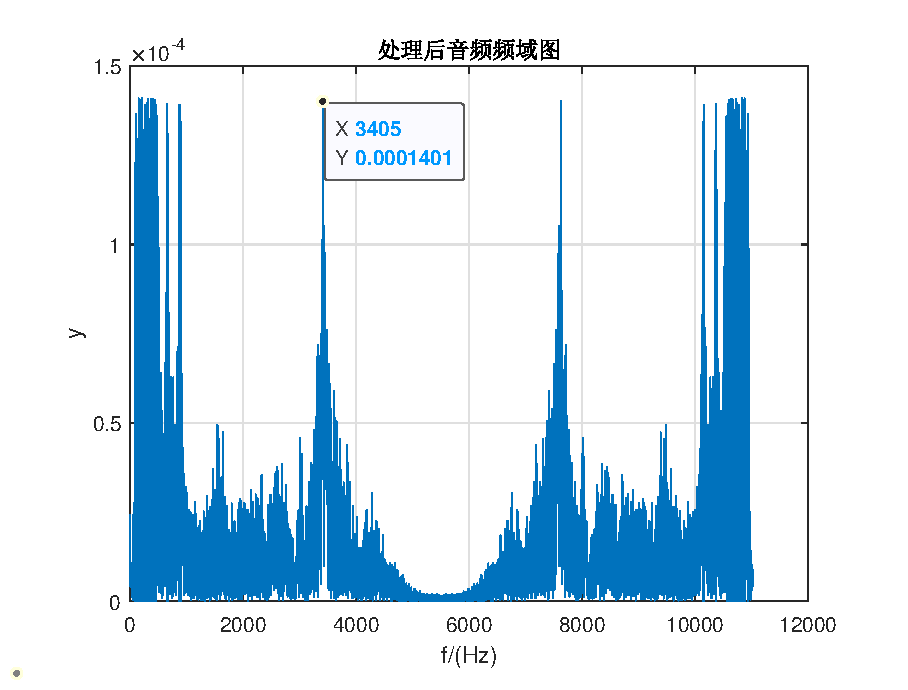
\includegraphics[width=11cm]{af-picf.eps}	
    }
    \hfill 
    \subcaptionbox{时域图}{
        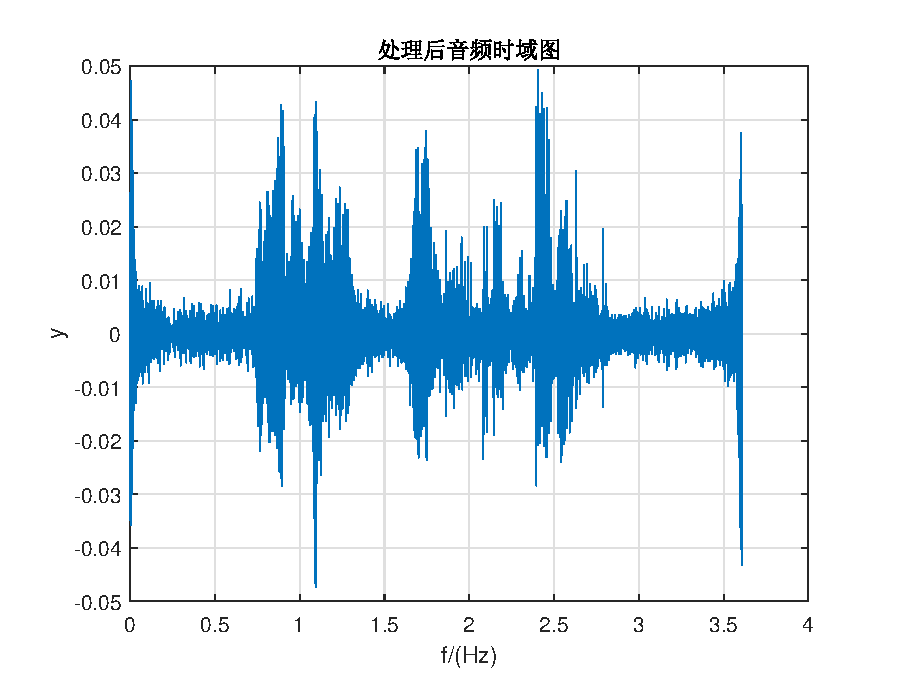
\includegraphics[width=11cm]{af-pict1.0.eps}	
    }
    \caption{一次处理后音频信号频域域图}
\end{figure}
\newpage
$\bullet$但是,第一步处理后听到处理音频仍伴随着持续低噪声,考虑使用带通滤波器直接去除双边频域信号.观测时域图也可发现,时域音频的‘毛刺’明显减少\\
\indent 此时持续低噪声明显消失,但此时人声听起来‘失真’,效果稍显不佳。\textit{(与初步处理音频相比更不像真人说话的效果,可以认为处理效果较为不佳)}

\begin{figure}[H]
    \centering
    \subcaptionbox{处理音频信号频域图}{
        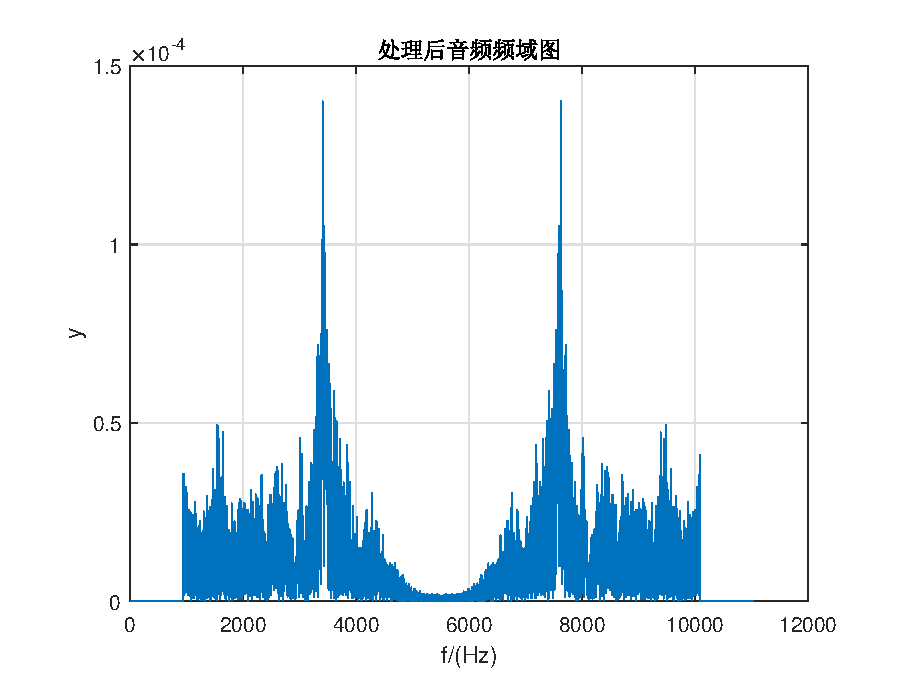
\includegraphics[width=11cm]{af-picf0.eps}	
    }
    \hfill 
    \subcaptionbox{处理音频信号时域图}{
        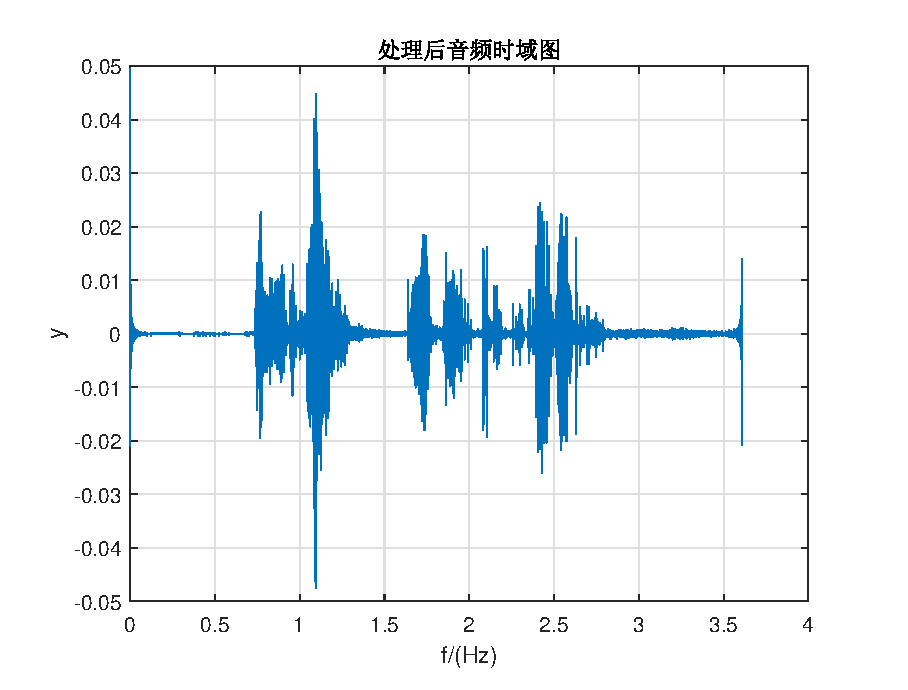
\includegraphics[width=11cm]{af-pict0.0.eps}	
    }
    \caption{全部滤波处理后音频信号频域域图}
\end{figure}
\newpage
$\bullet$ 人声听起来‘失真’,会不会是因为被滤去的双侧信号中仍含有部分音频信息呢?\\
\indent 于是,取双侧信号进行频域、时域分析,声音处理后仍可勉强辨识出,男声:‘这里是电子科技大学’。\\
\indent 不过,此时人声清晰度明显不足,且伴有较大噪声。但是仍可从此次变换中得到双侧\textbf{信号仍包含重要信息不应该被简单置零}的结论。\\
\begin{figure}[H]
    \centering
    \subcaptionbox{频域图}{
        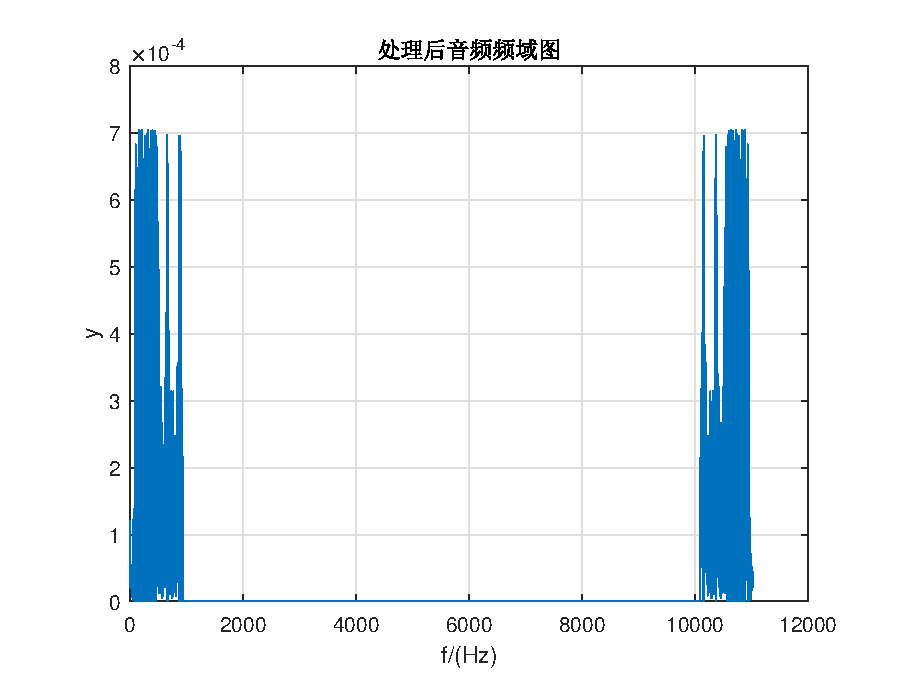
\includegraphics[width=10cm]{111.eps}	
    }
    \hfill 
    \subcaptionbox{时域图}{
        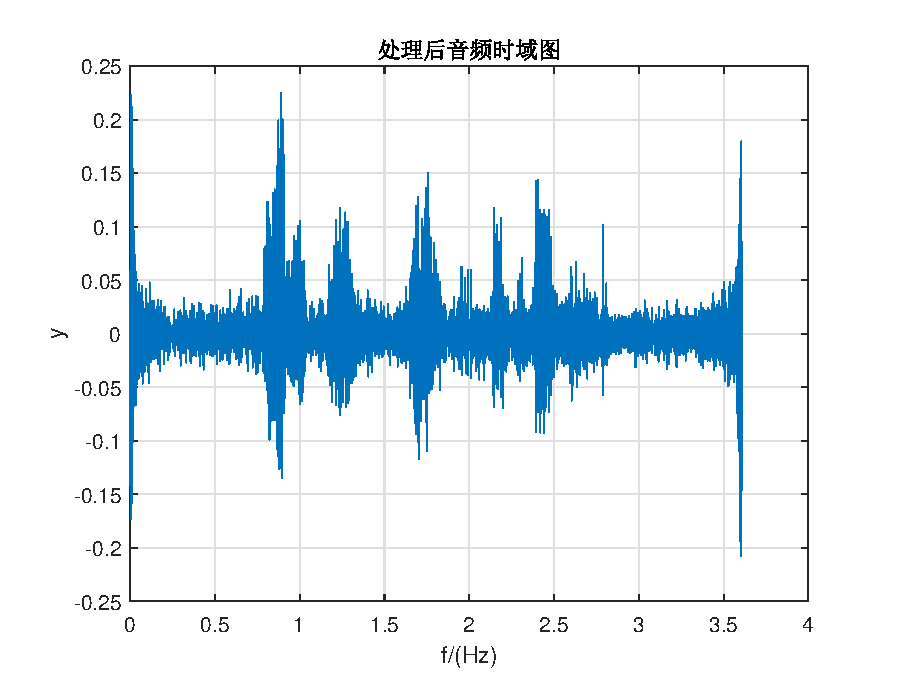
\includegraphics[width=10cm]{112.eps}	
    }
    \caption{双侧音频信号频域域图}
\end{figure}
$\bullet$ 那么可以知道双边频率信号的存在会带来与人声音量相近的持续低噪声,但是会使人声听起来‘更饱和’,于是考虑对双侧信号进行幅度调整减小噪音音量,而非直接滤除。\textit{【此部分噪声在单音噪声之间表现为没有个性的毛刺,故判断此段为宽频噪声,通过资料查询,可以使用幅度调制进行消减】}
\begin{figure}[H]
    \centering
    \
    \subcaptionbox{幅度调整为0.1倍-【频域】}{
        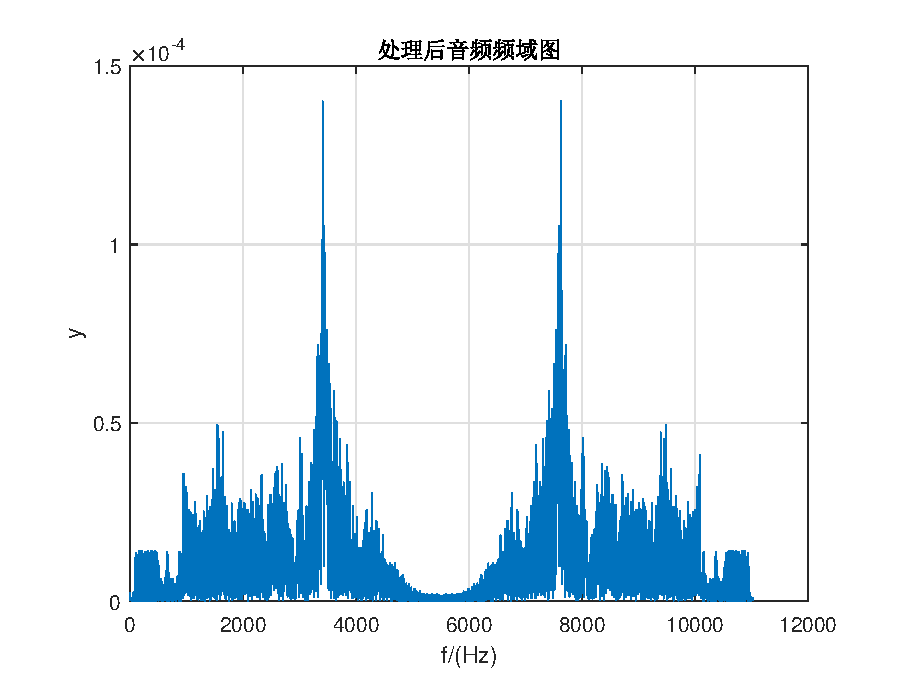
\includegraphics[width=7.2cm]{af-picf0.1.eps}	
    }
    \hfill 
    \subcaptionbox{幅度调整为0.1倍-【时域】}{
        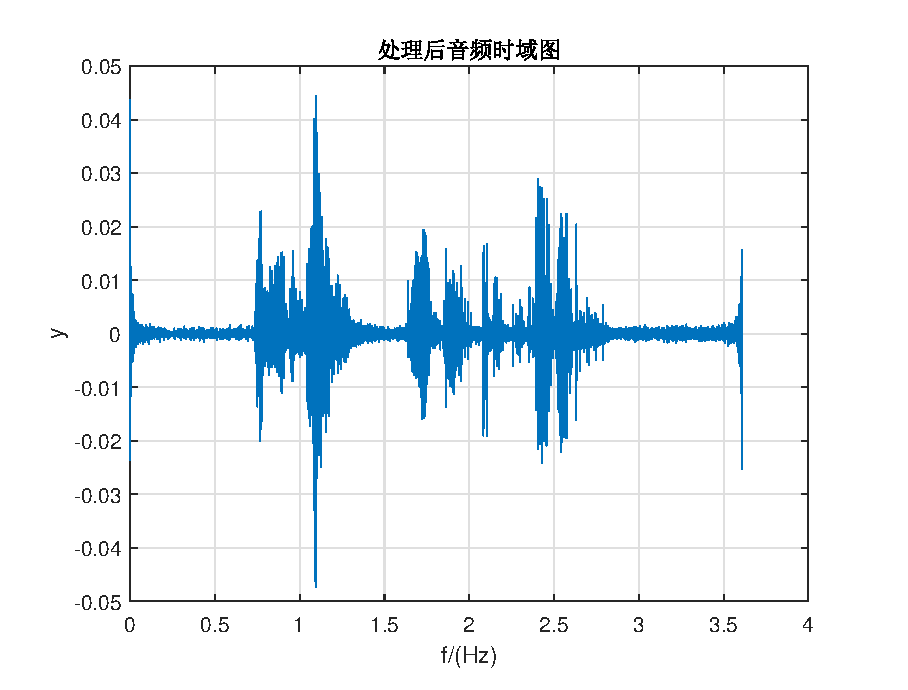
\includegraphics[width=7.2cm]{af-pict0.1.eps}	
    }
    \hfill 
    
    \subcaptionbox{幅度调整为0.5倍-【频域】}{
        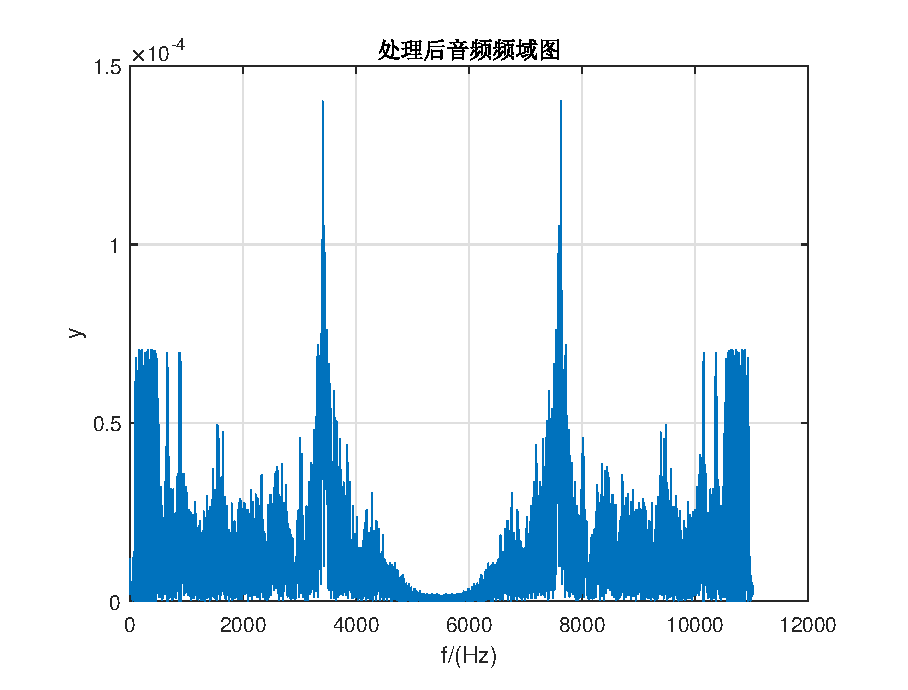
\includegraphics[width=7.2cm]{af-picf0.5.eps}	
    }
    \hfill 
    \subcaptionbox{幅度调整为0.5倍-【时域】}{
        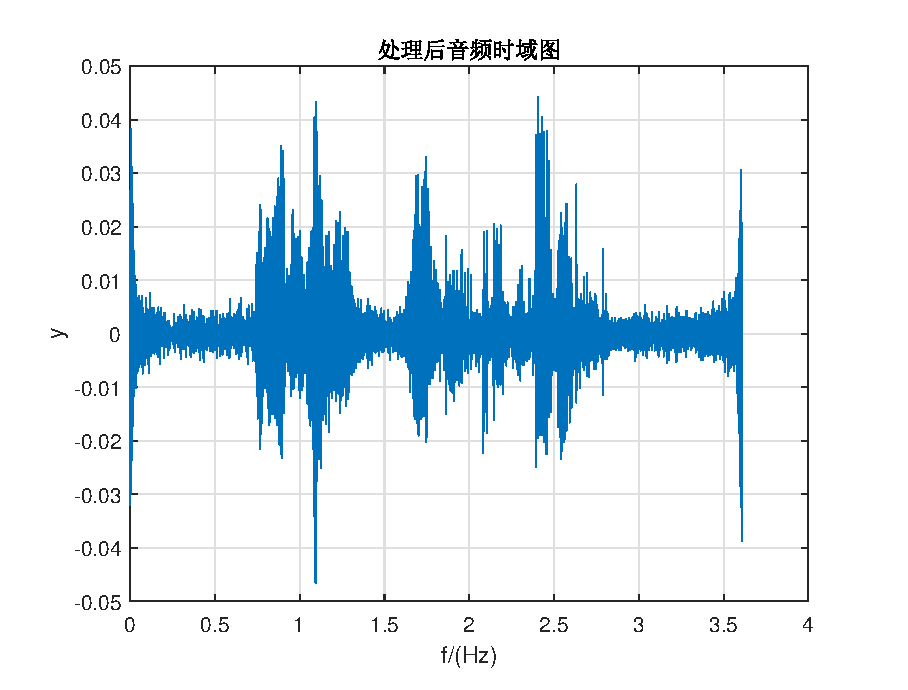
\includegraphics[width=7.2cm]{af-pict0.5.eps}	
    }
    \hfill 
    \subcaptionbox{幅度调整为0.8倍-【频域】}{
        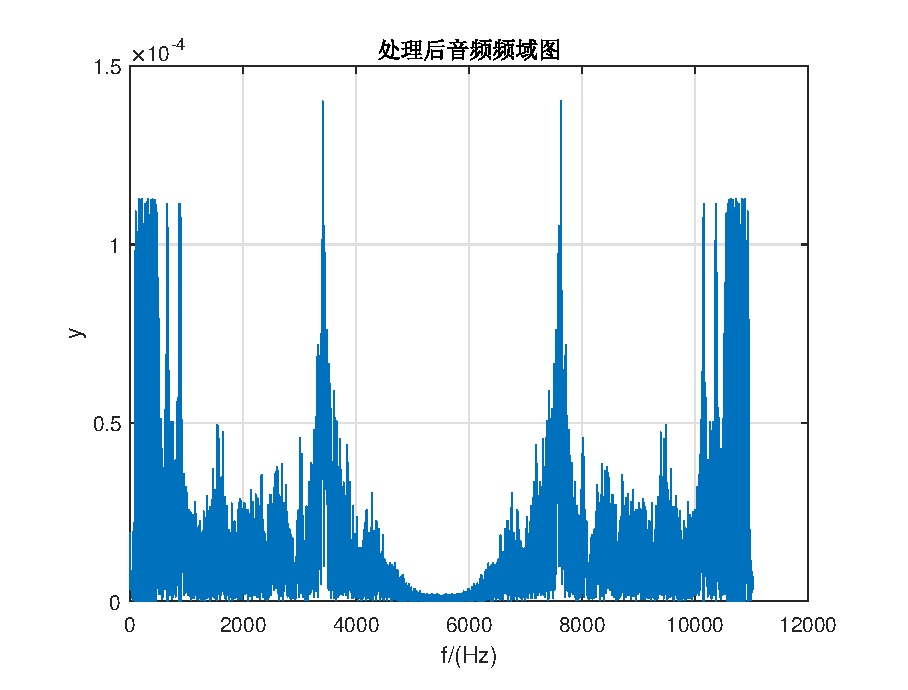
\includegraphics[width=7.2cm]{af-picf0.8.eps}	
    }
    \hfill 
    \subcaptionbox{幅度调整为0.8倍-【时域】}{
        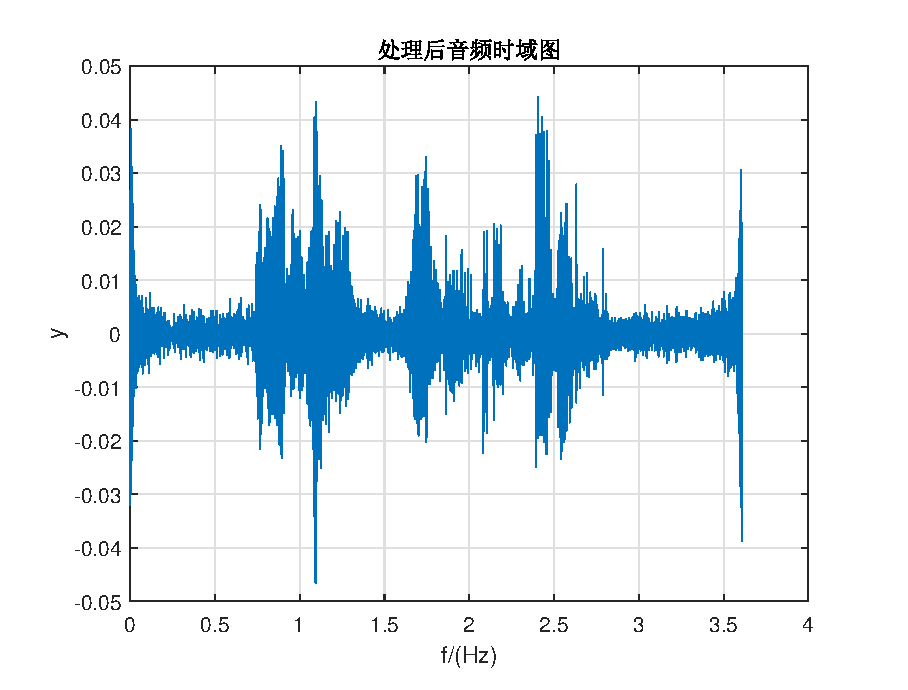
\includegraphics[width=7.2cm]{af-pict0.8.eps}	
    }
    \caption{多次测试-双侧信号幅度调制}
\end{figure} 
$\bullet$ 经过多次尝试,将幅度调整0.2倍时,可以保持人声的‘饱和’同时消减持续低噪声。此时,可认为目前去噪效果呈现为\textbf{最佳状态:可听出音频中男声‘这里是电子科技大学’,且音频噪声较小且人声饱满贴近真实声音}。
\begin{figure}[H]
    \centering
    \subcaptionbox{频域图}{
        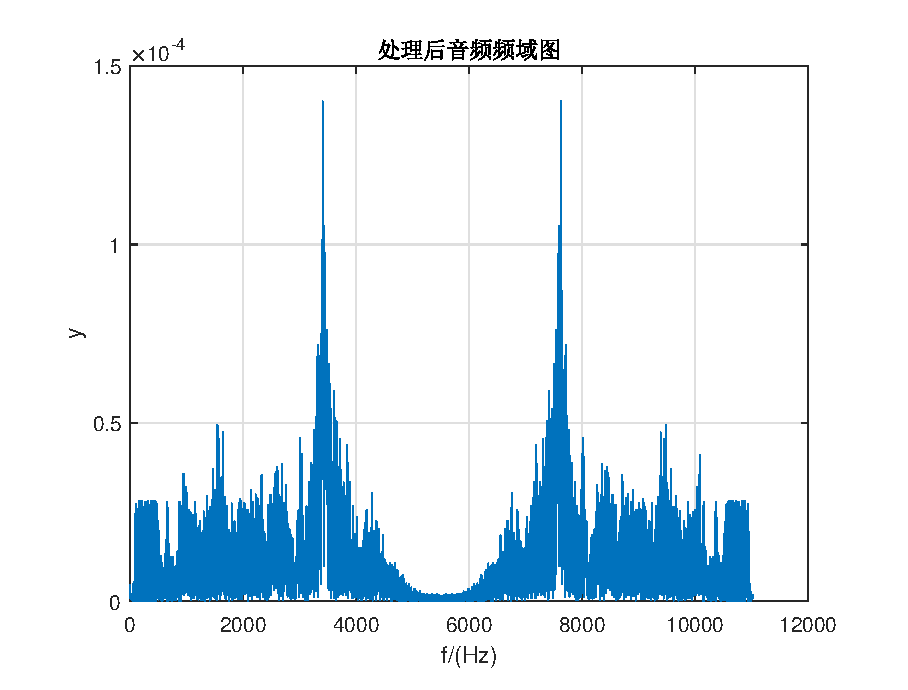
\includegraphics[width=11cm]{af-picf0.2.eps}	
    }
    \hfill 
    \subcaptionbox{时域图}{
        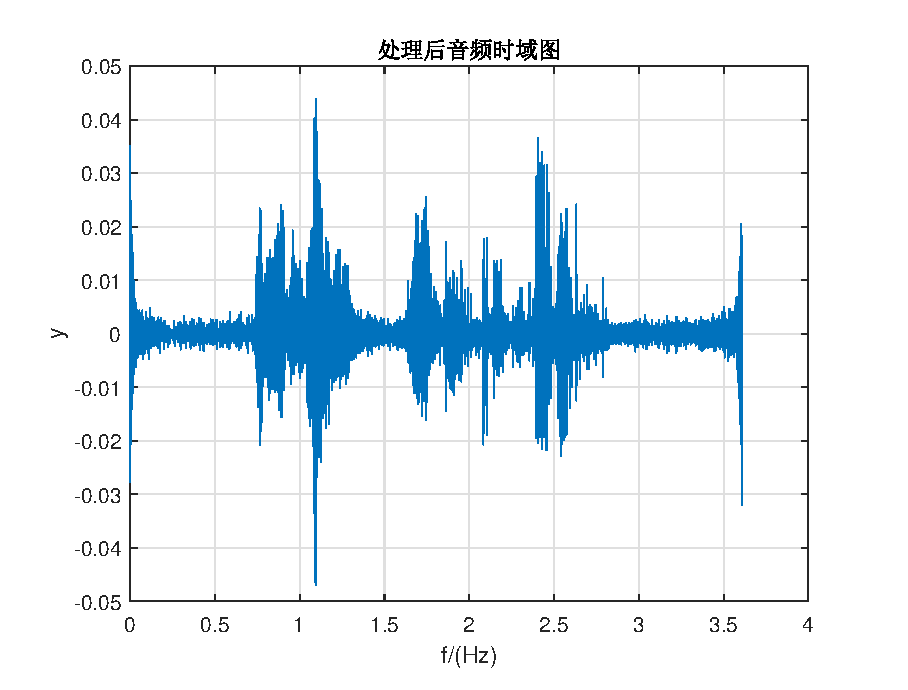
\includegraphics[width=11cm]{af-pict0.2.eps}	
    }
    \caption{最佳处理所得音频信号}
\end{figure}